\documentclass{article}

\usepackage{amsmath}
\usepackage{amssymb}
\usepackage{graphicx}



% bold letters
\newcommand{\bola}{\mathbf{a}}
\newcommand{\bolc}{\mathbf{c}}
\newcommand{\bolf}{\mathbf{f}}
\newcommand{\bolg}{\mathbf{g}}
\newcommand{\boll}{\mathbf{l}}
\newcommand{\bolq}{\mathbf{q}}
\newcommand{\bolp}{\mathbf{p}}
\newcommand{\bolu}{\mathbf{u}}
\newcommand{\bolv}{\mathbf{v}}
\newcommand{\bolw}{\mathbf{w}}
\newcommand{\bolz}{\mathbf{z}}

\newcommand{\bolA}{\mathbf{A}}
\newcommand{\bolB}{\mathbf{B}}
\newcommand{\bolC}{\mathbf{C}}
\newcommand{\bolD}{\mathbf{D}}
\newcommand{\bolE}{\mathbf{E}}
\newcommand{\bolF}{\mathbf{F}}
\newcommand{\bolG}{\mathbf{G}}
\newcommand{\bolH}{\mathbf{H}}
\newcommand{\bolI}{\mathbf{I}}
\newcommand{\bolJ}{\mathbf{J}}
\newcommand{\bolK}{\mathbf{K}}
\newcommand{\bolL}{\mathbf{L}}
\newcommand{\bolM}{\mathbf{M}}
\newcommand{\bolN}{\mathbf{N}}
\newcommand{\bolO}{\mathbf{O}}
\newcommand{\bolP}{\mathbf{P}}
\newcommand{\bolQ}{\mathbf{Q}}
\newcommand{\bolR}{\mathbf{R}}
\newcommand{\bolS}{\mathbf{S}}
\newcommand{\bolT}{\mathbf{T}}
\newcommand{\bolU}{\mathbf{U}}
\newcommand{\bolV}{\mathbf{V}}
\newcommand{\bolW}{\mathbf{W}}
\newcommand{\bolX}{\mathbf{X}}
\newcommand{\bolY}{\mathbf{Y}}
\newcommand{\bolZ}{\mathbf{Z}}

% bold symbols
\newcommand{\bolalpha}{\boldsymbol{\alpha}}
\newcommand{\bolbeta}{\boldsymbol{\beta}}
\newcommand{\boleta}{\boldsymbol{\eta}}
\newcommand{\bolpsi}{\boldsymbol{\psi}}

% shadowed letters
\newcommand{\PP}{\mathbb{P}}
\newcommand{\RR}{\mathbb{R}}
\newcommand{\CC}{\mathbb{C}}
\newcommand{\ZZ}{\mathbb{Z}}

% mathcal letters
\newcommand{\calA}{\mathcal{A}}
\newcommand{\calB}{\mathcal{B}}
\newcommand{\calC}{\mathcal{C}}
\newcommand{\calD}{\mathcal{D}}
\newcommand{\calE}{\mathcal{E}}
\newcommand{\calF}{\mathcal{F}}
\newcommand{\calG}{\mathcal{G}}
\newcommand{\calH}{\mathcal{H}}
\newcommand{\calI}{\mathcal{I}}
\newcommand{\calJ}{\mathcal{J}}
\newcommand{\calK}{\mathcal{K}}
\newcommand{\calL}{\mathcal{L}}
\newcommand{\calM}{\mathcal{M}}
\newcommand{\calN}{\mathcal{N}}
\newcommand{\calO}{\mathcal{O}}
\newcommand{\calP}{\mathcal{P}}
\newcommand{\calQ}{\mathcal{Q}}
\newcommand{\calR}{\mathcal{R}}
\newcommand{\calS}{\mathcal{S}}
\newcommand{\calT}{\mathcal{T}}
\newcommand{\calU}{\mathcal{U}}
\newcommand{\calV}{\mathcal{V}}
\newcommand{\calW}{\mathcal{W}}
\newcommand{\calX}{\mathcal{X}}
\newcommand{\calY}{\mathcal{Y}}
\newcommand{\calZ}{\mathcal{Z}}


% derivatives
\newcommand{\pp}[2]{\frac{\partial #1}{\partial #2}}
\newcommand{\dd}[2]{\frac{d #1}{d #2}}


% fraction shortcut
\newcommand{\f}[2]{\frac{#1}{#2}}
\newcommand{\slfrac}[2]{\left.#1\middle/#2\right.}

% common operators
\newcommand{\vvvert}{|\kern-1pt|\kern-1pt|}
\newcommand{\enorm}[1]{\vvvert #1 \vvvert}


% matrices
\newcommand{\bmat}[1]{\left(\begin{array}{#1}}
\newcommand{\emat}{\end{array}\right)} 



\newcommand{\blist}{\begin{list}{\ballrefb}{\leftmargin=2.0em}
  \setlength{\itemsep}{2pt}
  \setlength{\parskip}{0pt}}
\newcommand{\elist}{\end{list}}



% common format strings
\def\etal{{\it et al.}}
\def\ie{{\it i.e.}}
\def\eg{{\it e.g.}}


\DeclareMathOperator*{\arginf}{arg\,inf}
\DeclareMathOperator*{\argsup}{arg\,sup}
\DeclareMathOperator*{\argmax}{arg\,max}
\DeclareMathOperator*{\argmin}{arg\,min}


\begin{document}
	\begin{center}
		\LARGE AER1418 Assignment 1 \\
		\normalsize Geoff Donoghue --- January \(17^{th}\) 2019
	\end{center}

\section*{Part I}
\begin{itemize}
	\item[(a)] We have two boundary conditions, one on \(\Gamma_\text{in} \) and one on \(\Gamma_\text{out} \), the condition on the former boundary is a Neumann boundary condition while the latter is a Robin boundary condition. Both of these can be taken to be natural boundary conditions, (and therefore not enforced by the choice of space). This allows us to take both our test and trial spaces to be 
	\begin{equation}
		\calV_0 \equiv H^1(\Omega_\text{annulus}).
	\end{equation}
	In order to determine the linear and bilinear forms we will apply the weighted residual method, first multiplying by some test function \(v \in \calV_0\) then integrating over \(\Omega_\text{annulus} \) to obtain
	\begin{equation}
		0 = \int_{\Omega_\text{annulus}} v \left( -\nabla \cdot \left(k\nabla u \right)\right) dx.
	\end{equation}
	Integration by parts yields
	\begin{equation}
		0 = \int_{\Omega_\text{annulus}} \nabla v \cdot k\nabla u dx - \int_{\Gamma_\text{in}} v\left(\hat{n} \cdot k\nabla u \right)dl - \int_{\Gamma_\text{out}} v\left(\hat{n} \cdot k\nabla u \right)dl,
	\end{equation}
	where \(\hat{n}\) represents the outward pointing unit normal vector and \(dl\) is a line element along the boundary. Incorporating the conditions along each boundary in the above equation yields
	\begin{equation}
		0 = \int_{\Omega_\text{annulus}} \nabla v \cdot k\nabla u dx - \int_{\Gamma_\text{in}} vg dl + \int_{\Gamma_\text{out}} v\left(B_\text{out}\left(u - u_\infty \right) \right)dl.
	\end{equation}
	By taking \(u_\infty = 0\), and defining \(a_0(w,v)\) and \(\ell_0(v)\) to be
	\begin{align}
		a_0(w,v) &\equiv \int_{\Omega_\text{annulus}} \nabla v \cdot k\nabla w dx + \int_{\Gamma_\text{out}} B_\text{out}vw dl,\\
		\ell_0(v) &\equiv \int_{\Gamma_\text{in}} vgdl.
	\end{align}
	We arrive at the weak formulation of our problem: find \(u \in \calV_0\) such that
	\begin{equation}
		a_0(u,v) = \ell_0(v) \quad \forall v \in \calV_0.
	\end{equation}
	
	\item[(b)] By noting the radial symmetry of our problem we can choose to reexpress the integrals in our weak form in terms of polar coordinates \(\left(r,\theta\right) \). By doing so we obtain \(dx = rdrd\theta, \text{ and }dl = rd\theta \), we also note that the symmetry of the problem implies \(\pp{u}{\theta} = 0 \). Applying these changes to our weak form, we obtain 
	\begin{equation}
		0 = \int_{\Omega_\text{annulus}} k\dd{v}{r}\dd{u}{r} rdrd\theta - \int_{\Gamma_\text{in}} vg rd\theta + \int_{\Gamma_\text{out}} B_\text{out}vu rd\theta. 
	\end{equation}
	Noting further independence of \(\theta\) we can divide the equation by \(2\pi\) and define \(\Omega \equiv \left(r_\text{in},r_\text{out} \right) \subset \RR \), this yields
	\begin{equation}
		0 = \int_{\Omega} k\dd{v}{r}\dd{u}{r} rdr -  \left[vgr\right]_{r = r_\text{in}} + \left[B_\text{out}vur \right]_{r=r_\text{out}}. 
	\end{equation}
	Following this we note that we still have natural boundary conditions and can therefore define our test and trial function spaces to both be
	\begin{equation}
		\calV \equiv H^1\left(\Omega\right).
	\end{equation}
	Our weak formulation may then finally be expressed as: find \(u \in \calV \) such that
	\begin{equation}
		a(u,v) = \ell(v) \quad \forall v \in \calV,
	\end{equation}
	where we define \(a(w,v)\) and \(\ell(v) \) as 
	\begin{align}
		a(w,v) &\equiv \int_{\Omega} k\dd{w}{r}\dd{v}{r} rdr + B_\text{out}r_\text{out}v(r_\text{out})w(r_\text{out}) \\ 
		\ell(v) &\equiv  gr_\text{in}v(r_\text{in}).
	\end{align}
	
	\item[(c)] We wish to show that \(\exists\alpha \) such that \(a(v,v) \geq \alpha\|v\|^2_\calV, \; \forall v \in \calV \equiv H^1(\Omega) \). We begin by expanding the \(H^1\left(\Omega\right)\) norm
	\begin{equation}
		\|v\|^2_{H^1(\Omega)} = |v|^2_{H^1(\Omega)} + \|v\|^2_{L^2(\Omega)}.
	\end{equation}
	Since \(\Omega \subset \RR, \Gamma_\text{out} \subset \partial\Omega, \text{ and } \Gamma \neq \emptyset\), the Poincar\'e-Friedrichs inequality can be applied to the final term in the preceding equation, yielding
	\begin{align}
		\|v\|^2_{H^1(\Omega)} \leq& \;|v|^2_{H^1(\Omega)} + C_\text{PF}\left(|v|^2_{H^1(\Omega)} + \|v\|^2_{L^2(\Gamma_\text{out})}  \right)\\
		\leq& \left(1+C_\text{PF}\right) |v|^2_{H^1(\Omega)} + C_\text{PF}v(r_\text{out})^2.
	\end{align}
	Without changing the value on the right side of the inequality we can say that 
	\begin{equation}
		\|v\|^2_{H^1(\Omega)} \leq \left(1+C_\text{PF}\right) \int_\Omega \left(\dd{v}{r}\right)^2 dr + C_\text{PF}\dfrac{B_\text{out}r_\text{out}} {B_\text{out}r_\text{out}}v(r_\text{out})^2.
	\end{equation}
	Since our domain \(\Omega \) is strictly positive we can also say that
	\begin{equation}
		\|v\|^2_{H^1(\Omega)} \leq \left(1+C_\text{PF}\right) \dfrac{1}{kr_\text{in}}\int_\Omega kr\left(\dd{v}{r}\right)^2 dr + C_\text{PF}\dfrac{B_\text{out}r_\text{out}} {B_\text{out}r_\text{out}}v(r_\text{out})^2.
	\end{equation}
	Finally we note that we have each term in our bilinear form, without knowing which is larger we can say that
	\begin{equation}
		\|v\|^2_{H^1(\Omega)} \leq \max\left\{\left(1+C_\text{PF}\right) \dfrac{1}{kr_\text{in}} , C_\text{PF}\dfrac{1} {B_\text{out}r_\text{out}}\right\}a(v,v).
	\end{equation}
	Thereby showing that our bilinear form is coercive with a coercivity constant
	\begin{equation}
		\alpha = \left(\max\left\{\left(1+C_\text{PF}\right) \dfrac{1}{kr_\text{in}} , C_\text{PF}\dfrac{1} {B_\text{out}r_\text{out}}\right\} \right)^{-1}.
	\end{equation}
	
	\item[(d)] In order to show that the bilinear form is continuous in \(H^1(\Omega) \) we must show that \(\exists\gamma \) such that 
	\begin{equation}
		a(w,v) \leq \gamma \|w\|_{H^1(\Omega)}\|v\|_{H^1(\Omega)}.
	\end{equation}
	We begin with the definition of the bilinear form and apply the trace inequality
	\begin{align}
		a(w,v) =& \int_\Omega k \dd{w}{r}\dd{v}{r}rdr + B_\text{out}r_\text{out}w(r_\text{out})v(r_\text{out})\\
			=& \int_\Omega k \dd{w}{r}\dd{v}{r}rdr + B_\text{out}r_\text{out} \|w\|_{L^2(\Gamma_\text{out})} \|v\|_{L^2(\Gamma_\text{out})}\\
			\leq& \int_\Omega k \dd{w}{r}\dd{v}{r}rdr + B_\text{out}r_\text{out}C_\text{tr}^2 \|w\|_{H^1(\Omega)} \|v\|_{H^1(\Omega)} \\
			\leq& \;kr_\text{out}  |w|_{H^1(\Omega)}|v|_{H^1(\Omega)} + B_\text{out}r_\text{out}C_\text{tr}^2 \|w\|_{H^1(\Omega)} \|v\|_{H^1(\Omega)}.
	\end{align}
	We note that since \(|w|_{H^1(\Omega)}|v|_{H^1(\Omega)} \leq \|w\|_{H^1(\Omega)}\|v\|_{H^1(\Omega)}\) we can say that 
	\begin{equation}
		a(w,v) \leq \max\left\{kr_\text{out}, B_\text{out}r_\text{out}C_\text{tr}^2 \right\}\|w\|_{H^1(\Omega)}\|v\|_{H^1(\Omega)},
	\end{equation}
	which demonstrates continuity of the bilinear form in \(H^1(\Omega)\) with a continuity constant
	\begin{equation}
		\gamma \equiv \max\left\{kr_\text{out}, B_\text{out}r_\text{out}C_\text{tr}^2 \right\}.
	\end{equation}
	
	\item[(e)] A linear form is continuous in \(\calV \equiv H^1(\Omega) \) if \(\exists c \) such that
	\begin{equation}
		|\ell(v)| \leq c\|v\|_{H^1(\Omega)}.
	\end{equation}
	Starting from the definition of our linear form, we may apply the trace inequality to obtain
	\begin{align}
		|\ell(v)| =&\; |gv(r_\text{in})r_\text{in}| \\
			=&\; gr_\text{in} \|v\|_{L^2(\Gamma)} \\
			\leq&\; g r_\text{in} C_\text{tr} \|v\|_{H^1(\Omega)}.
	\end{align}
	We therefore say our linear form is continuous. 
	
	\item[(f)] Since our bilinear form is both continuous and coercive on our test and trial space \(\calV \equiv H^1(\Omega) \), our linear form is continuous on \(H^1(\Omega) \), and our domain \(\Omega \) is a Lipschitz domain, we simply apply the Lax-Milgram theorem which states that our variational problem has a unique solution. 
	
	\item[(g)] If we update our Biot number such that \(B_\text{out} = 0\), our bilinear form becomes
	\begin{equation}
		\tilde{a}(w,v) \equiv \int_{\Omega} k\dd{v}{r}\dd{u}{r} rdr.
	\end{equation}
	In order to show that the updated bilinear form \(\tilde{a} \) is not coercive we will show that the coercivity condition is violated for constant functions. We let \(v = c \neq 0 \), with \(c\) being some arbitrary nonzero constant over \(\Omega \) (we note by definition \(v\in H^1(\Omega) \)). By choosing constant \(v\) we obtain
	\begin{equation}
		\tilde{a}(v,v) = \int_\Omega k \left(\dd{c}{r}\right)^2 = \int_\Omega k \left(0\right)^2 rdr = 0,
	\end{equation}
	and
	\begin{equation}
		\|v\|^2_{H^1(\Omega)} = \int_\Omega \left(\dd{c}{r}\right)^2 + c^2 dr =  \int_\Omega c^2 dr = \|c\|^2_{L^2(\Omega)} > 0.
	\end{equation}
	The last inequality is strict because \(c\) is itself nonzero. Since we have \(\tilde{a}(v,v) < \|v\|^2_{H^1(\Omega)}\) the bilinear form is not coercive if \(B_\text{out} = 0 \). In order to show that this form admits many unique solutions, let us suppose that \(u\) is some solution to our variational problem, satisfying
	\begin{equation}
		\tilde{a}(w,v) \equiv \int_{\Omega} k\dd{v}{r}\dd{u}{r} rdr = gv(r_\text{in})r_\text{in} = \ell(v).
	\end{equation}
	Let us define \(\tilde{u} \equiv u + c \), where \(c\) is again some arbitrary nonzero constant defined as before. We note that there are infinitly many \(\tilde{u} \) that can be defined this way. We see that \(\tilde{a}(u,v) = \tilde{a}(\tilde{u},v) \), and that there are therefore infinitely many solutions to the bilinear form when the Biot number is zero. 
	
	\item[(h)]	Since our bilinear form was shown to be coercive and is symmetric by inspection we may define a minimization formulation of our problem by first defining our function space to be the same as before \(\calV_0 \equiv H^1(\Omega_\text{annulus}) \) and defining an energy functional \(\calJ : \calV_0 \to \RR \) as
	\begin{equation}
		\calJ(w) = \dfrac{1}{2}a_0(w,w) - \ell_0(w) =  \quad \forall w \in \calV_0.
	\end{equation}
	% \dfrac{1}{2}\left(\int_{\Omega_\text{annulus}} \nabla v \cdot k\nabla u dx - \int_{\Gamma_\text{in}} v\left(\hat{n} \cdot k\nabla u \right)dl \right) + \int_{\Gamma_\text{out}} v\left(\hat{n} \cdot k\nabla u \right)dl
	We will therefore seek a solution \(u \in \calV_0 \) such that 
	\begin{equation}
		u = \argmin\limits_{w\in\calV_0} \calJ(w).
	\end{equation}
	
\end{itemize}

\section*{Part II}

\begin{itemize}
	\item[(a)] See attached.
	
	\item[(b)] Figure \ref{soln} shows the solution to the variational problem with the specified parameters. 
	\begin{figure}[t]
		\centering
		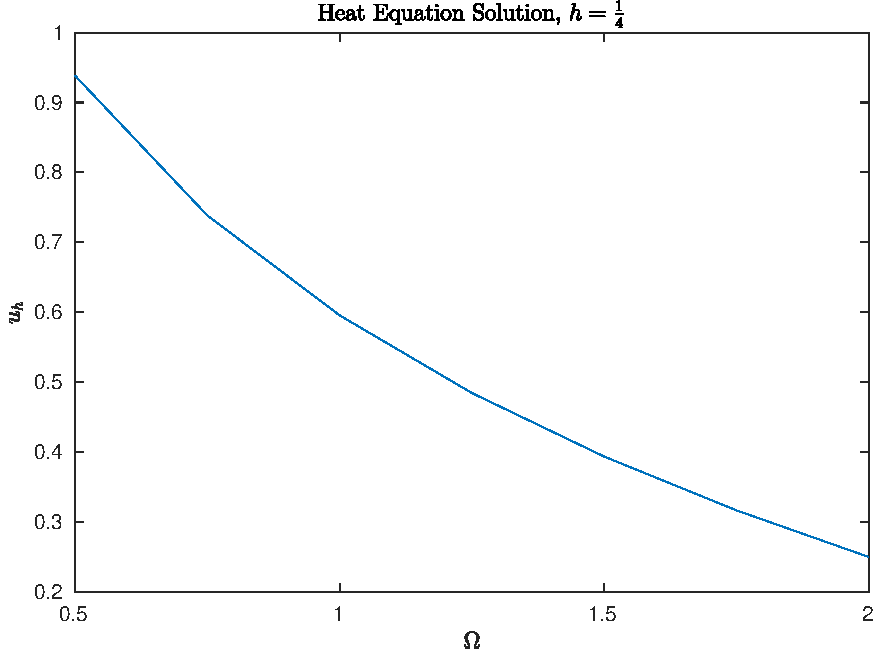
\includegraphics[width=0.85\textwidth]{fig2.pdf}
		\caption{Solution field to heat problem, with \(h = \frac{1}{4} \).}
		\label{soln}
	\end{figure}
	
	\item[(c)] We begin by applying Galerkin orthogonality to the bilinear form \(a(e,e)\)
	\begin{equation}
		a(e,e) \equiv a(u-u_h,u-u_h) = a(u,u-u_h) - \underbrace{a(u_h,u-u_h)}_{=0 \forall u_h \in \calV_h \subset \calV}.
	\end{equation}
	From here, we say that \(a(u,v) = l(v) \forall v \in \calV \), and note that \(\ell^\text{o}(w) = \ell(w) \forall w \in \calV  \)
	\begin{equation}
		a(e,e) = a(u,u-u_h) = \ell(u-u_h).
	\end{equation}
	Since \(\ell \) is a linear form we can relate the error in the finite element approximation of the solution to the error in the output as follows
	\begin{equation}
		a(e,e) = \ell(u-u_h) = \ell(u) - \ell(u_h) = \ell^\text{o}(u) - \ell^\text{o}(u_h),
	\end{equation}
	which yields the desired relation. 
	
	\item[(d)] Figure \ref{conv} plots the error in the output with respect to the highly refined reference solution on a log-log scale. The convergence rate is was determined to be
	\begin{equation}
		r = \dfrac{\log\left(e_{h=1/64}/ e_{h=1/32} \right)}{\log\left((1/64) / (1/32) \right)} = 2.0163
	\end{equation}
	\begin{figure}[t]
		\centering
		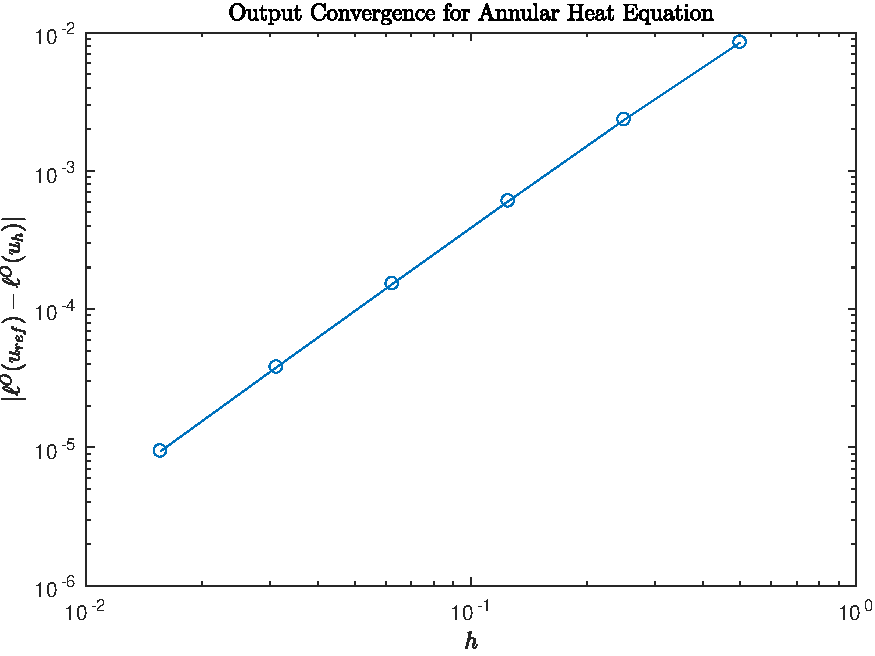
\includegraphics[width=0.85\textwidth]{fig1.pdf}
		\caption{Solution field to heat problem, with \(h = \frac{1}{4} \).}
		\label{conv}
	\end{figure}
	Which is in agreement with the expected rate of \(r = 2\), for the square of the energy norm, for linear finite elements.
\end{itemize}
	
\end{document}